\chapter{Evaluation} 
This chapter presents an evaluation of the initial results from the collected data focusing on statistics relating to
developmental trajectories in order to identify potential developmental indices. These findings serve as the
foundation
for the feature selection used in training the explainable boosting machine. Features that demonstrate strong
performance here may also be identified as important by the EBM. The following questions will be addressed in this
section:

\begin{enumerate}
    \item Which measures show an overall developmental trajectory across JLPT levels?
    \item Which features significantly discriminate between proficiency levels, and is a developmental trajectory
    apparent across these levels?
\end{enumerate}

\section{Complexity Measures}

Many of the complexity measures demonstrated trends that correspond to increasing proficiency. However, the patterns
varied across measures. Some showed a consistent increase,while others
decreased, or plateaued at the
higher levels. Notably, most measures were unable to distinguish between the N1 and native speaker (NS) groups.

Statistical analyses were conducted using ANOVA to test for significance, followed by Tukey's HSD test to identify
significant pairwise differences between adjacent proficency levels.

\subsection{Syntactic Complexity Measures}

%Sentence Length
    %discriminates between ajacent proficency levels.
%Clause per Sent
    %*Statistically significant difference between all adjacent levels except N1 and NS

Many of syntactic measures failed to show significant differences between N1 and NS groups. However several measures
such as sentence length, clauses per sentence, and coordinating clauses per sentence exhibited statistical significance
across most
adjacent proficency levels. These patterns are illustrated in Figures \ref{fig:sentLen}, \ref{fig:cpersent}, and
_____ respectively.

\begin{figure}[htbp]
    \centering
    \begin{minipage}{.48\textwidth}
        \centering
    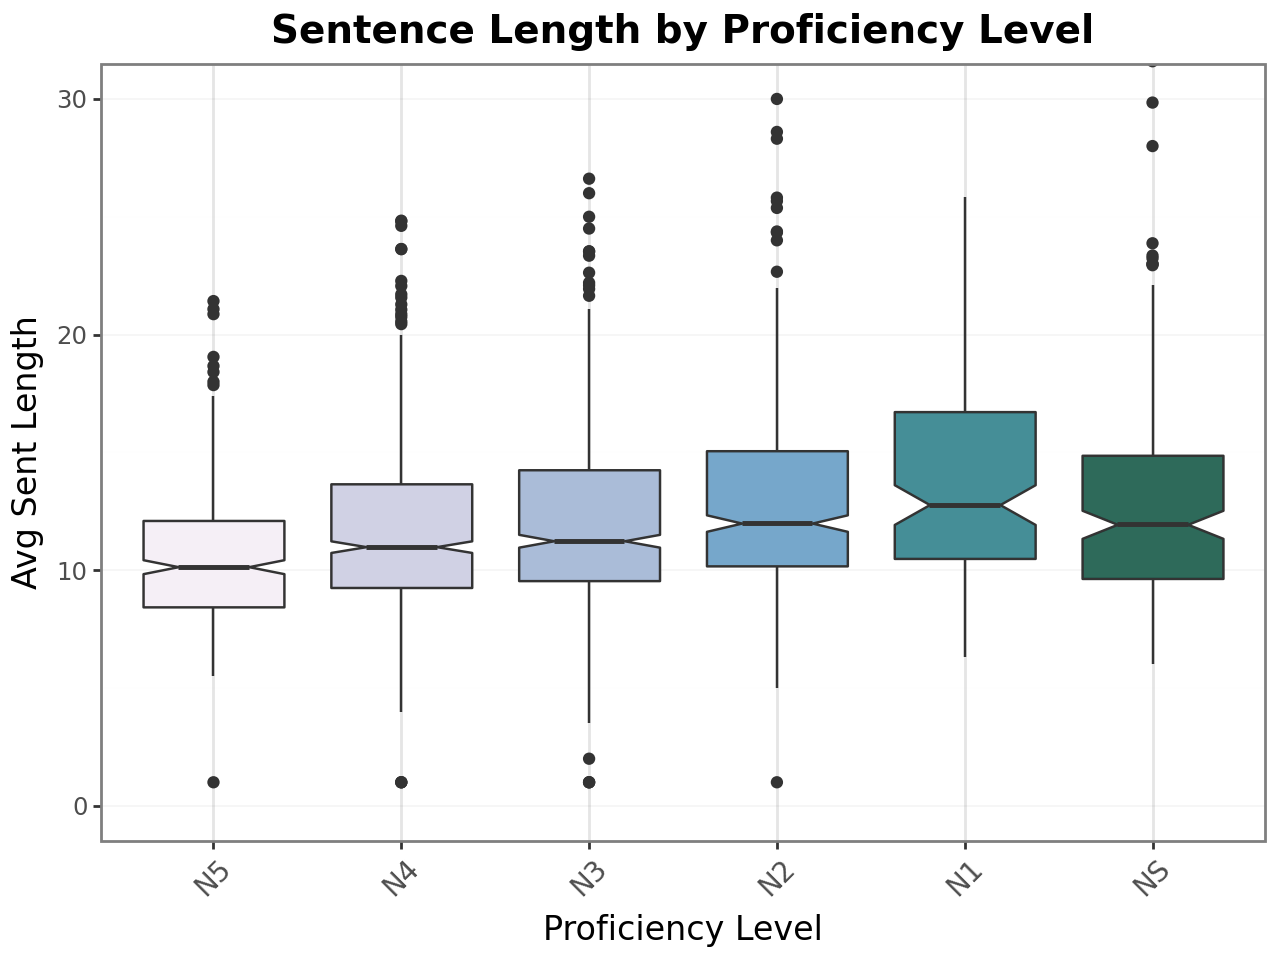
\includegraphics[scale=.3]{img/sentence_len}
    \caption[Average Sentence Length across JLPT levels]{}
        \label{fig:sentLen}
    \end{minipage}
    \hfill
\begin{minipage}{.48\textwidth}
        \centering
        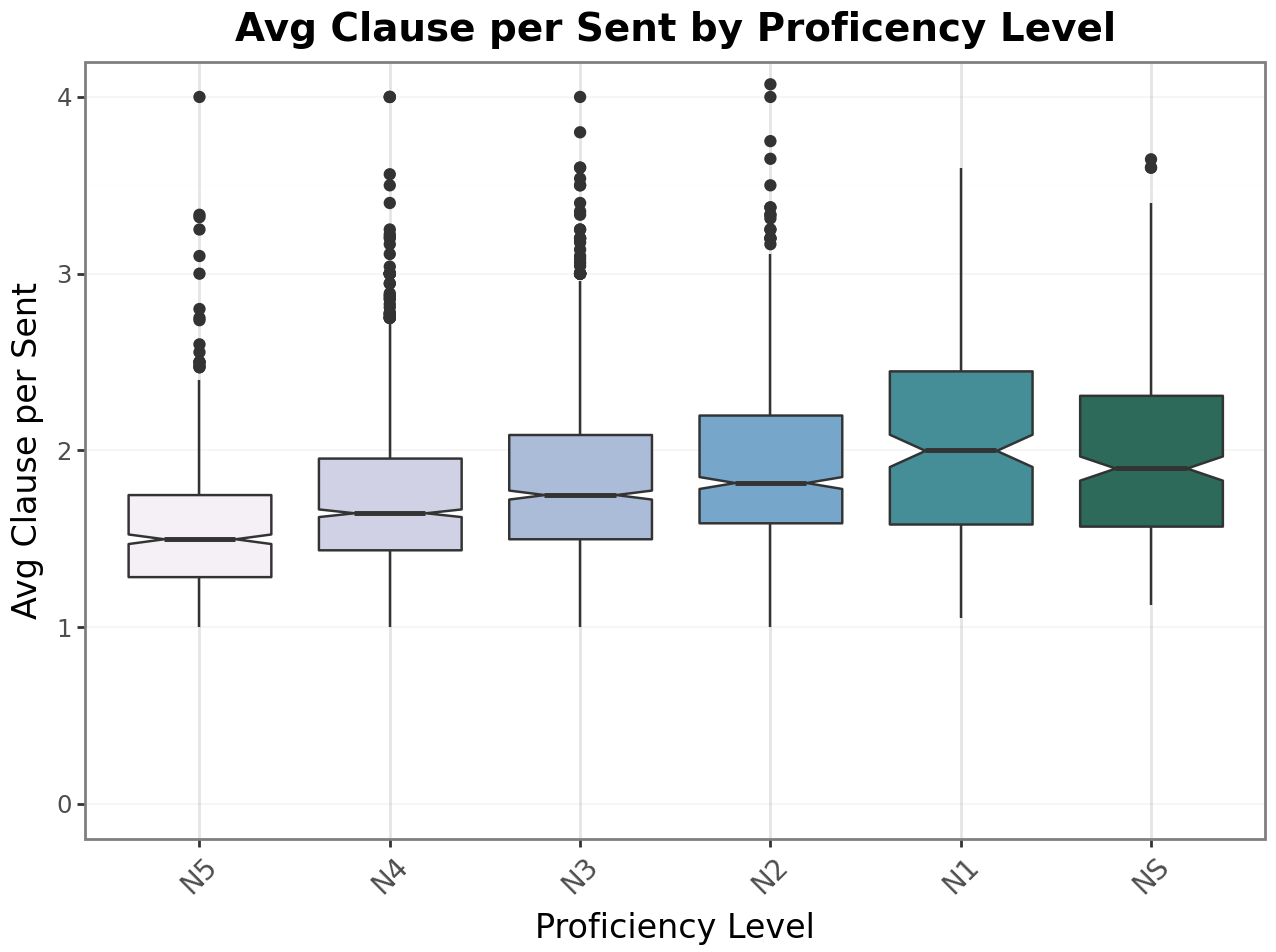
\includegraphics[scale=.3]{img/clausesSent}
        \caption{Plot showing the ratio of clauses per sentence}
\label{fig:cpersent}
\end{minipage}
    \end{figure}


\subsubsection{Length-Based Measures}

Length-based metrics capture the amount of syntactic material produced per unit (e.g. per sentence, per clause,
etc.) and are surface level-indications of syntactic complexity. Sentence length exhibited a general upward trend
across proficiency levels and was statistically significant at distinguishing across most adjacent levels, although
it failed to distinguish N1 from the NS group. This aligns
with
the idea that more advanced learners integrate more elements into a single sentence.

Clause length showed slight
increases and a significant difference in distinguishing between N1 and N3 levels, this could be sensitive to task
or possibly developed in the higher proficiency levels.
%TODO check between tasks


Noun phrase length and verb phrase legnth in constrast were less informative. NP length remained relatively stable
and did not significantly differ across levels. Verb phrase length did show a weak upward trend but lacked
statistical significance to distinguish between the proficency levels.

\subsubsection{Clause-Based Measures (Including Coordination/Subordination)}

Across previous studies on language development and complexity
measures a decreasing trend of coordination and increase in subordination was observed but my findings demonstrate
the opposite.



Subordinating Conjunction per Sent
    statistically significance difference between N5 and N4 but does not discriminate between the higher proficency
    levels. Subordination is taught quite early to L2 speakers, could this be why?
Subordinating Conjunction per clause
    statistically significant difference between N5 and N4 and N4 and N3,
Coordinating Conjunction per Sentence
    *Statistically significant in distinguishing all adjacent levels except N1 and NS group
    *Also increases across prof levels, could be due to the fact that SC are taught first.
Coordinating Conjunction per Clause
    *increase across prof. levels
    *Statistically significant between levels except N2 & N1 and N1 & NS
Subordinating Clauses to Coordinate Clauses
    *statistically significant for every other proficency level. ie. N5 & N3, N3 & N1, N2&N4
    *variance also increases at the higher proficency levels but , maybe due to more CC being used?
CC Freq
    no significant difference between any of the levels and no clear pattern...
SC Frequency
    *increases across levels
    *Significant between n5&N4, N4&N3, N3&N2, N2 & NS
Clause Length
    *N1 and N3 statistically significant difference observed
    *slightly increases across levels.
    *Could be influenced by tasks?. Try Removing SW1 and SW2 tasks

\subsubsection{Dependency-Based Measures}

MDD
    * Statistically significant between every other level as well as the higher proficency levels N3&N2 and N2&N1
    *no significant between N1 and NS
    *Increase across levels
MHD
    *Increase across levels
    *statistically significant between all adjacent levels except NS and N1


\subsection{Lexical}
CTTR
    *Discriminates between adjacent levels at the lower proficiency levels,but no statistical significant difference
    found between N2 & N1 and N1 & NS, and N2 and NS
    *Generally increases between levels
MTLD-Surface
    * increases across levels
    * Statistically significant in distinguishing between lower prof levels.('N2', 'N3'), ('N2', 'N4'), ('N3', 'N5'), ('N4','N5')
MTLD-Inflection
    *increases across levels not as much as with surface forms
    * Statistically significant in distinguishing between lower prof levels.('N2', 'N3'), ('N2', 'N4'), ('N3', 'N5'), ('N4','N5')
Noun Density
    *Decreases across proficiency levels (null subjects?)
    *distinguishes beteween lower prof levels. N4 & N5 and N3 and N4 (almost significant p = .06)
Verb Density
    *increase across levels
    * Only statistically significant at distinguishing between lower levels N5 & N4 and N4&N3
Adjective Density
    *Increase across proficiency levels
    *Statistically significant in distinguishing between lower levels N5&N4, N5&N3, N3&N2
    *could also be task dependent check later
Adverb Density
    *increase across levels except a drop in use for N1 (due to low sample size?)
    *Statistically significant in distinguishing between lower levels N4&N5, N3&N5 N3&N2
LFP

LFP -BWCCJ Corpus
    * high frequency of items in top 1,000 band across all proficiency levels
    *N1 and Ns group had the largest raw count of vocab used across each band
    * However,

LFP - JLPT WordList
    *

\subsection{Morphological}
*MCI - Surface vs. Lemma
\subsubsection{MCI Measures}
MCI 5-Surface
\begin{itemize}
   \item *46 texts removed
   \item  *Increase across levels
    \item *statistically significant across groups except N1&NS and N1 and N2
 \end{itemize}
MCI 5-Inflection
    *46 texts dropped
    *not as great an increase across levels
    *does not discriminate between adjacent levels but every other level at lower levels N5&N3, N4&N2
MCI 10 - Surface (634 texts dropped)
    * Increase across levels
    * Statistically significant at lower levels N5 - N2 , no significance between N2, N1, NS
MCI 10 - Inflection
    *statistically significant difference between N1 and NS!
    *Statistically significant at lower levels N5-N2, no significance between N2 and N1

*Conclusion the surface/standard calculation is enough and yields more statistically significant results.MCI10
results in more learner texts being dropped due to length. MCI5 is more than enough when working with lower
proficiency learners.
\subsubsection{JRMA Measures}
JRMA Measures

*MTLD measures had dropped texts due to the minimum text length limit required. This is especially true for
these measures as it is using specific function/content words meaning even longer text is needed.


JRMA_all_MTLD
    *49 rows removed
    *statistically significant difference in distinguishing N5&N4, N3&N2 levels

JRMA_function_MTLD
    *2377 rows removed
    * only difference in N4 and N3 were statistically significant.
    *no clear pattern of increasing/decreasing

JRMA_content_MTLD
    * 2446 rows removed of 4840
    * Statistically significant in distinguishing the lower levels. N4&N5 N3&N2
*
JRMA_all_MATTR
    *Significant difference between all levels except the N1&NS,and N1&N2
    * slight increase across levels, variance also decreases

JRMA_Function_MATTR
    *Slight decrease across levels.
    *decrease in variance across levels
    * significant pairs: (N5,N4), (N4,N3),(N5,N3)

JRMA_Content_MATTR
    * decrease in variance across levels
    * significant pairs: (N2,N3), (N5,N3)

Auxiliary Chains
    * significant pairs (N5,N4),(N3,N5)
    * increase from N5 to N4, but after that plateaus. Meaning that after the beginning levels chain size doesn't
    increase
\section{Criterial Features}
Raw counts of features, 
look at how many of structures from each level are used across all features used


possibly also include qualitative analysis on extracted grammar forms.?

Raw counts of grammar forms across all proficency levels (and native)

CF_tai_N5_total          1705
CF_ukemi_N4_total        1688
CF_toomou_N4_total       1586
CF_toiu_N3_total         1056
CF_tara_N4_total          948
CF_youni_N4_total         822
CF_tabini_N3_total        520
CF_tekudasai_N5_total     495
CF_saseru_N4_total        471
CF_tekuru_N4_total        333

\section{Task Effect}
Look into differences in results across tasks...